
\item In the figure, a ladder of mass $m$ is shown leaning against a wall. It is in static equilibrium making an angle $\theta$ with the horizontal floor. The coefficient of friction between the wall and the ladder is $\mu_1$ and that between the floor and the ladder is $\mu_2$. The normal reaction of the wall on the ladder is $N_1$ and that of the floor is $N_2$. If the ladder is about to slip, then
    \begin{center}
        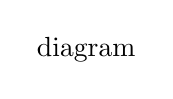
\begin{tikzpicture}
            \node at (0, 0) {diagram}; % "diagram" should be replaced with the actual file path of the image.
        \end{tikzpicture}
    \end{center}
    \begin{tasks}(2)
        \task $\mu_1 = 0 \quad \mu_2 \neq 0\quad$and$N_2 \tan\theta = \frac{mg}{2}$
        \task $\mu_1 \neq 0 \quad \mu_2 = 0\quad$and$N_1 \tan\theta = \frac{mg}{2}$
        \task $\mu_1 \neq 0 \quad \mu_2 \neq 0\quad$and$N_2 = \frac{mg}{1+\mu_1\mu_2}$
        \task $\mu_1 = 0 \quad \mu_2 \neq 0\quad$and$N_1 \tan\theta = \frac{mg}{2}$
    \end{tasks}
